%%
%% static_code_analysis_in_ci.tex
%% V0.1
%% 2015/01/22
%% by 
%% Sebastian Funke
%% Hamza Zulfiqar
%% Brian Pfretzschner
%% See:
%% https://github.com/hzulfiqar/SecSoftDev
%% for current contact information.
%%


\documentclass[conference]{IEEEtran}


% *** PACKAGES ***
%\usepackage{algorithmic}
%\usepackage{array}
%\usepackage{mdwmath}
%\usepackage{mdwtab}
%\usepackage{eqparbox}
%\usepackage{fixltx2e}
%\usepackage{stfloats}
\usepackage{cite}       % http://www.ctan.org/tex-archive/macros/latex/contrib/supported/cite/
\ifx\pdfoutput\undefined
\usepackage{graphicx}   % http://www.ctan.org/tex-archive/macros/latex/required/graphics/
\else
\usepackage[pdftex]{graphicx}
\fi
\usepackage{subfigure}  % http://www.ctan.org/tex-archive/macros/latex/contrib/supported/subfigure/
\usepackage{url}        % http://www.ctan.org/tex-archive/macros/latex/contrib/other/misc/
\usepackage[cmex10]{amsmath}    % http://www.ctan.org/tex-archive/macros/latex/required/amslatex/math/
%\usepackage{amsfonts}
\interdisplaylinepenalty=2500
\ifx\pdfoutput\undefined
\usepackage[hypertex]{hyperref}
\else                   % http://www.ctan.org/tex-archive/macros/latex/contrib/supported/hyperref/
\usepackage[pdftex,hypertexnames=false]{hyperref}
\fi
\usepackage[colorinlistoftodos,prependcaption,textsize=tiny]{todonotes}
\usepackage{listings}
\lstset{frame=single,captionpos=b}

% correct bad hyphenation here
\hyphenation{op-tical net-works semi-conduc-tor}

\begin{document}
%
% paper title
\title{An Evaluation of Open Source Static Code Analysis Reporting in Context of Continuous Integration Tools}



%\author{\IEEEauthorblockN{Sebastian Funke}
%\IEEEauthorblockA{Secure Software Engineering\\
%TU Darmstadt\\
%sebastian.funke@stud.tu-darmstadt.de}
%\and
%\IEEEauthorblockN{Brian Pfretzschner}
%\IEEEauthorblockA{Secure Software Engineering\\
%TU Darmstadt\\
%brian.pfretzschner@stud.tu-darmstadt.de}
%\and
%\IEEEauthorblockN{Hamza Zulfiqar}
%\IEEEauthorblockA{Secure Software Engineering\\
%TU Darmstadt\\
%hamza.zulfiqar@stud.tu-darmstadt.de}}



\author{\authorblockA{Sebastian Funke, Brian Pfretzschner, Hamza Zulfiqar}
	\authorblockA{Center for Advanced Security Research Darmstadt\\
		Department of Computer Science\\
		Technische Universit\"at Darmstadt, Germany}}




% use for special paper notices
%\IEEEspecialpapernotice{(Invited Paper)}




% make the title area
\maketitle


\begin{abstract}
Static code analysis should run frequently in a continuous integration lifecycle. Each run produces a lot of information that need to be reviewed, evaluated and integrated in the ongoing development process. Therefore, the analysis results should be reported in a clear and meaningful fashion. Additionally, results might be combined, reworked, concentrated or filtered. We use only open source tools that are freely available and examine how they work together and what their results look like.
\end{abstract}

% no keywords

% For peerreview papers, this IEEEtran command inserts a page break and
% creates the second title. It will be ignored for other modes.
\IEEEpeerreviewmaketitle



\section{Introduction}
\label{sec:introduction}
% no \IEEEPARstart
Building secure software systems gets more and more important. Not just private hackers are attacking our software, also foreign and even western governments put in great effort in breaking into important systems\cite{NSAHacking}. To do so, they need some kind of vulnerability to attack. Since writing vulnerability-free software is hard, tools are welcome to support and maintain software quality on an ongoing basis. Static code analysers can fulfil this task.


Continuous integration is a software development philosophy. The key idea is the entire software product is tested, built and measured after each commit. ``In essence, Continuous Integration is about reducing risk by providing faster feedback. First and foremost, it is designed to help identify and fix integration and regression issues faster, resulting in smoother, quicker delivery, and fewer bugs.''\cite{Jenkins:Smart:2011} Furthermore, one can think of additional tasks that can monitor software quality regularly. By doing so, it is possible to notice common problems or a degradation of code quality as soon as possible. This is a huge opportunity to reduce risk on a permanent basis.


Therefore, we have to improve the software development process in terms of early and continuous security analysis of the source code.
Such static analysis tools can be applied independently during the development process at different stages.
One option would be the integration of analysers into the Integrated Development Environment (IDE) of the developer.
Another possibility is the combination of those tools in a continuous integration system, to collect issues during or after the build process.
Besides CI and IDE the development tool chain can be extended with Code Quality Management systems, as platform for analyse the code and manage the analysed issues.


In our paper, we compare and evaluate the issue reporting capabilities in two CI tools (Jenkins and Teamcity), in a Code Quality Management tool (SonarQube) and in the IDE Eclipse.
We integrated the popular analysers FindBugs and PMD in each development tool above and executed them on a Java test project (JEdit\footnote{\href{http://www.jedit.org/}{JEdit: An open source text editor written in Java}}) with a variety of issues.


We motivated and introduced the idea of our work in the introduction \ref{sec:introduction}.
Next we explain the foundations of static code analysis in section \ref{sec:static_code_analysis} and \ref{subsec:static_code_analysis_foundations}, with the classification of lexical- and data flow analysis in section \ref{subsubsec:lex_analysis} and \ref{subsubsec:dataflow_analysis} respectively, and two popular analysers FindBugs and PMD which we used in our evaluation.

Then we differentiate between the possibilities where to apply static code analysis, in IDE's, CI systems and CQM systems in the sections \ref{sec:static_code_analysis_ide}, \ref{sec:static_code_analysis_ci} and \ref{sec:static_code_analysis_code_quality_management} and explain the levels of integration in CI for Jenkins in subsection \ref{subsec:ci_levels_of_integration}.
Thereby, we introduce the open source tools we evaluated: Eclipse (\ref{sec:static_code_analysis_ide}), Jenkins (\ref{subsec:jenkins}), Teamcity (\ref{subsec:teamcity}) and SonarQube (\ref{subsec:sonarqube}).

In our evaluation in section \ref{sec:evaluation} we decide for an evaluation strategy (\ref{subsec:walkthrough}), identify important evaluation questions for our evaluation walk-through (\ref{subsubsec:evaluation_prepare}, \ref{subsubsec:evaluation_run}, \ref{subsubsec:evaluation_results}, \ref{subsubsec:evaluation_manage}), explain our evaluation results for every tested tool in the subsections \ref{subsec:evaluation_eclipse}, \ref{subsec:evaluation_jenkins}, \ref{subsec:evaluation_teamcity} and \ref{subsec:evaluation_sonarqube} and create a matrix to compare the evaluated tools in subsection \ref{subsec:comparation}.


Finally we conclude our work in section \ref{sec:conclusion}.

\section{Static code analysis}
\label{sec:static_code_analysis}
\subsection{Overview}
\label{subsec:static_code_analysis_overview}
Static code or program analysis is an automated analysis performed on the static source code of a program without executing it \cite{Static_Code_Analysis_def}.
The aims are to enhance robustness and to find errors and all kind of programming mistakes early during the coding and testing phases, to reduce the effort of bug-fixing after the release of the software.


Analysers that execute the program and analyse the dynamic behaviour on the binaries are called dynamic code analysers.
Those analysers might be easier to implement, because they analyse the already loaded binaries and won't have to deal with complicated programming language features, like reflection and anonymous classes, but on the other hand, they are limited in their reporting capabilities.
Modern approaches try to combine both or try to break down the source code in a simpler immediate representation.
The analysis framework Soot\footnote{\href{https://sable.github.io/soot/}{Soot: A framework for analysing and transforming Java and Android Applications}} for example transforms complicated Java code into a three-operator code, called Jimple and allows to implement analysers on an easier representation.
However, dynamic or hybrid code analysers are out of scope for this work and not further mentioned.


Especially for low-level programming languages like C, static code analysis became a crucial part of software development to find memory leaks and other coding mistakes.
Hence, it is used automatically in compilers to find rough programming mistakes and most common security flaws.
Anyway, detailed or special purpose security analysers can't be part of a compiler, they need to be applied externally with custom rules to decrease the number of false positives and to increase development performance.

Typical types of analysis do:
\begin{itemize}
	\item Type checking
	\item Style/Code quality checking
	\item Program/Property verification
	\item Pointer, buffer, file and memory checking
	\item Control flow management
	\item Initialization and shutdown checks
\end{itemize}

Increasing the precision (less false positive) and performance, as well as decreasing the recall (less false negatives) of analysers is the prevailing goal of the research in this area and characterizes the quality of a static code analyser.


\subsection{Foundations and Classification}
\label{subsec:static_code_analysis_foundations}
There are different types of analysers which all have a different scope. Most of them are specialized to a specific programming language, but some are also capable of analysing multiple languages. An example for a multi-language analyser is CPD\footnote{\href{http://pmd.sourceforge.net/pmd-4.3.0/cpd.html}{CPD: Copy/Paste Detector}} which is supposed to find duplicate code. It works with Java, JSP, C, C++, Fortran and PHP code.


On a very high level, all analysers share a common way of performing a static analysis, as shown in figure \ref{fig:analysis}.
They parse, tokenize and lex the source code and build a context free grammar, just like a compiler does.
Out of that, they build an abstract model, for example an Abstract Syntax Tree (AST).
Finally, they use external rules and security knowledge to perform the analysis on the built model and display the results in a human readable way.

\begin{figure}[!t]
	\centering
	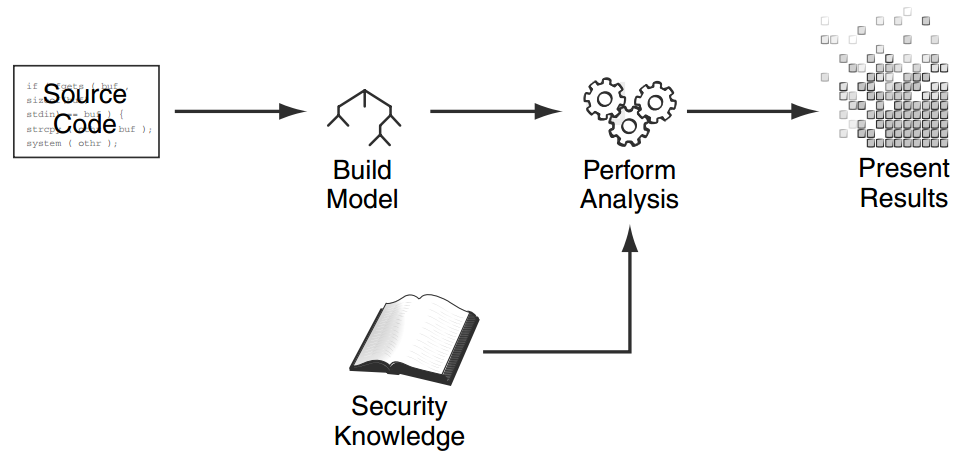
\includegraphics[width=1\linewidth]{img/analysis.png}
	\caption{Basic model of static code analysis \cite{Static_code_analysis_book_Chess:2007}}
	\label{fig:analysis}
\end{figure}

It is possible to differentiate two kinds of analysis, lexical- and data flow analysis.


\subsubsection{Lexical Analysis}
\label{subsubsec:lex_analysis}


The most analysers do a form of lexical analysis.
They build a model like an AST with symbol tables, analyse nodes against specific rules and use pattern matching to find anomalies and bugs.
An early and simple example from 2001 for such an analyser is the Rough Auditing Tool for Security (RATS)\cite{Static_code_analysis_book_Chess:2007}, now acquired by the successful commercial tool Fortify\footnote{\href{http://www8.hp.com/de/de/software-solutions/application-security/}{Fortify: Static code analyser by HP}}, that finds security and memory flaws in C source code, by doing a lexical analysis with XML-style rules, that contain already detailed descriptions of the corresponding problem.


\subsubsection{Dataflow Analysis}
\label{subsubsec:dataflow_analysis}


A data flow analysis uses additional models, like a \textit{Data Flow}- and \textit{Control Flow Graph (CFG)}, to find potential vulnerabilities and anomalies, by tracking data from inputs/sources to a leak/sink.
Typical analysis of that type are called Taint- or Live Variable Analysis.
The easiest approach of such an analyser operates only in a single function body (\textit{intra-procedural}).
Depending on the desired goal, such analysis can be \textit{flow-sensitive} (forward or top-down approach), to get control flow information about the past with more precision, or can be \textit{flow-insensitive} (backward or bottom-up approach), to get information about the future, but with less precision.


To extend the analysis scope to other functions, classes and packages (\textit{inter-procedural}), and automatically cover the different caller and callee contexts (\textit{context-sensitivity}) of a whole program with variable aliases and other language features, additional models, like \textit{Call Graphs}, \textit{Point-To-Sets} and \textit{Inter-procedural Control Flow Graph's} are necessary.
Examples for sophisticated inter-procedural analysers are Coverity\footnote{\href{https://www.coverity.com}{Coverity: Commercial inter-procedural static code analyser}} and FlowDroid\footnote{\href{http://sseblog.ec-spride.de/tools/flowdroid}{FlowDroid: Context-, flow-, field-, object-sensitive and lifecycle-aware static taint analysis tool for Android applications}} from Eric Bodden at the TU Darmstadt.
With modern language features like reflection, virtual dispatch and multi-threading, static code analysis become more and more complex, hence the performance and/or precision decreases.


FindBugs and PMD implement a data flow analysis and they are the open source static analysers we used later in our work for the evaluation.
Hence, they are described now.

\paragraph{PMD}
Is a source code analyser for Java, JavaScript, XML and XSL to find common programming flaws like unused variables, empty catch blocks, unnecessary object creation, etc.
It uses a set of rules, specified in a Java or XPath language, on an AST and a control flow graph with data flow nodes to produce a report with rule violations in XML format.


\paragraph{FindBugs}
Analyses Java class files for programming defects and uses nearly 300 bug patterns with different categories (bad practice, correctness, etc.) and severity classes (high, medium and low)\cite{Findbugs}.
Unlike PMD, it is possible to write custom detectors in Java as plugins to analyse java-bytecode or source code.
The detectors use techniques like visitor patterns over class files, with state-machines to save types, stack-values, constants and other information and by traversing the control flow graph, to save conditional information.
The FindBugs detectors are usually not inter-procedural, but do an additional global analysis to get knowledge about variables scopes and subtype-relationships.


Now it is important to distinguish when to apply analysers in a Software Development Lifecycle.
Most analysers, like FindBugs and PMD, exist as stand-alone version and allow the integration in common development tools, like IDE's, CI systems or Code Quality Management systems.




%\section{Input validation in popular frameworks}
%\label{sec:input_validation}
%\todo{Move this section to the end? - Brian}
%Check those \url{http://codegeekz.com/20-best-php-frameworks-developers-august-2014/} and make a table how input validation is handled there...
%The most common security weakness in any application is the failure to properly validate input from the environment. This weakness further leads to almost all of the major vulnerabilities in applications, including buffer overflow, SQL injection and a whole lot more. So, the maximum essential cautious measure that developers can take is to comprehensively authenticate the input that a software obtains. Certainly programs need to accept input, and computing a decent result depends on having a good input. There is a misconception that input can be trusted just because it is coming from some so-called trusted source. Input must not enter into the system without passing through various security methods.



\section{Static code analysis in IDE}
\label{sec:static_code_analysis_ide}
It is straightforward to integrate common analysers like PMD and FindBugs in an Integrated Development Environment (IDE) like Eclipse\footnote{An official list of Source Code Analysis plugins for Eclipse can be found in the \href{http://marketplace.eclipse.org/taxonomy/term/14,31}{Eclipse Marketplace}.}, Netbeans or IntelliJ.

With IDE (Integrated Development Environment), we mean a program ``that provides comprehensive facilities to computer programmers for software development. An IDE normally consists of a source code editor, build automation tools and a debugger.''\footnote{\href{http://en.wikipedia.org/wiki/Integrated_development_environment}{Integrated development environment}}
The IDE is usually the program that programmers use to develop new code, review code or fix bugs and issues. Since the programmer is used to navigate through the source using the IDE, it would be very helpful to enrich this environment by additional information. In contrast, reviewing analysis results in an independent and specialized program or website, code formatting and navigation can differ dramatically. Also, when it comes to fixing an issue, already being in the IDE means, a programmer can just make its changes instead of switching programs and locating the corresponding code location.

Static code analysis on IDE level is a common choice for many projects. Since the compiler does many static analysis, it is effectively integrated into any IDE that can start the compile process and interprets that compilers output.

Advantages of integrating additional static code analysers in IDEs:
\begin{itemize}
	\item Live feedback during programming
	\item Easy mapping of issues to code
	\item Possibility to fix issues early and instantly
	\item Reviewing and editing of source in one environment
	\item Interactive education for developers
	\item Extensibility thorough project specific rules
\end{itemize}

However disadvantages arise in bigger projects, especially data flow analysers, tend to scale not very well. 
There is no central way to configure the analyser rules, to improve the results and performance.
Many developers tend to suppress warnings from such analyzers, since they produce a lot of false positives.
Hence, it is desired to have a central and independent analyser, which can run on the remote repository code regularly and with predefined settings.

In this paper, we used the popular open source IDE Eclipse\footnote{\href{https://eclipse.org/}{https://eclipse.org/}}.
We decided for Eclipse because it is platform independent and highly extensible. Furthermore, we could integrate our test analysers PMD and FindBugs into Eclipse. Therefore, the results are comparable with the other platforms we evaluated.


\section{Static code analysis in CI}
\label{sec:static_code_analysis_ci}
Continuous Integration (CI) firstly proposed by Grady Booch \cite{CI-Definition:Booch:1993}, is the software engineering practice of continuously merging all developers working copies with a shared release master branch several times a day.

Advantages and disadvantages of Continuous Integration (CI)\cite{SecurityinCI}:
\begin{itemize}
	\item[+] \textit{Immediate Notification}:\\
	CI ensures that ongoing changes to the source code do not break the intent or design of the software. If a change does break the software, that break is identified immediately and can be fixed with a minimal cost and impact to the projects schedule.
	\item[+] \textit{Automated Testing and Deploying}:\\
	CI enables many automation possibilities. The most useful automation area is testing in form of Unit- and Integration-Testing, to find problems after component integration and change introduced bugs in previously working components. 
	Finally, a correct configured CI system can automate the deployment of software releases. 
	\item[+] \textit{Secure Development}:\\
	By integrating security testing and secure code analysis, CI can be further leveraged to include secure development practices while minimizing the amount of extra effort required to get the benefits of secure development. Since it is tied to CI,
	security testing and secure code review begins when a project begins and runs continuously
	throughout project development. With CI, vulnerability testing becomes part of the regression test bed, executed automatically with each successive build on the CI platform.
	
	\item[+] \textit{Changing Testing Economics}:\\
	Using CI for build, test, and analysis automation has increased the depth and breadth of tests while also making them faster and less expensive. By making it cheap and easy to perform tests, teams are encouraged to test more and test sooner in the development cycle, reducing the cost of fixing bugs.
	
	\item[+] \textit{Trend and History}:\\
	CI enables a higher management layer to view the history and trend of issues and builds.
	
	\item[-] \textit{CI Configuration}:\\
	The configuration of a CI instance can be very troublesome and involves the understanding of many different tools. To create a working tool chain of testing, analysing and building, with many thresholds and parameters the developer team has to understand every tool and have to tune parameters after gaining more experience.
\end{itemize}



\subsection{Levels of Integration}
\label{subsec:ci_levels_of_integration}
Depending on how continuous integration is accomplished in a given process management, static code analysis can be performed at different \textit{locations}, times and with different automation and reporting levels. According to \cite[p. 6ff]{Jenkins:Smart:2011}, there are \textit{7 phases} of applying continuous integration to a specific development. For this overview, only 3 phases apply: \textit{Phase 1} there is no common build server, \textit{Phase 2} there is a build server but builds run on a fixed (nightly) schedule and \textit{Phase 7} builds and tests (including analysis, measures) are issued as changes are committed.

\begin{itemize}
	\item[1] \textit{No Build Server} \\
	When no common build server exists, code analysis can only be applied on each developer's local machine. No developer is obliged to run the static code analysis before committing his changes nor will anybody be notified if code quality was decreased or new issues were introduced.
	
	
	\item[2] \textit{Nightly Builds} \\
	The build server could also run static code analysis and quality measures at each build and publish the results. Even notifications are possible, although they would not be accurately addressed since the system does not know which commit introduced the issue and can therefore not just notify the appropriate author.
	
	\item[3] \textit{Continuous Integration Environment} \\
	The server runs all tests, analyses and code measures at each commit, publishes the results and notifies the appropriate developer when the build failed or new issues were introduced through his change.
\end{itemize}



\subsection{Jenkins}
\label{subsec:jenkins}
Jenkins is a widely used tool to control and manage continuous integration tasks. Its main purpose is to monitor the execution of repeated jobs and present their outcomes\footnote{From Jenkins Website, \href{https://wiki.jenkins-ci.org/display/JENKINS/Meet+Jenkins}{Meet Jenkins}}.

We decided for Jenkins because it is open source, highly extensible and the most popular CI tool. To be exact, there are more than 1000 freely available plugins that can be installed by just one click using the Jenkins web interface.
Beside PMD and FindBugs, there are many more static analysers available in the plugin repository.
In our research we found, almost every analyser has a Jenkins plugin available.
Many OpenSource analysers, like BrakeMan\footnote{\href{http://brakemanscanner.org/}{http://brakemanscanner.org/}}, Cppcheck\footnote{\href{http://cppcheck.sourceforge.net/}{http://cppcheck.sourceforge.net/}} as well as popular commercial tools like Coverity\footnote{\href{http://www.coverity.com/}{http://www.coverity.com/}} and Fortify\footnote{\href{http://www8.hp.com/de/de/software-solutions/application-security/}{http://www8.hp.com/de/de/software-solutions/application-security/}}.
But not all plugins provide a full analyser.
Especially plugins for commercial tools like Coverity just provide a link to a corresponding web platform for code quality and issue management. 


%\begin{figure}[!t]
%	\centering
%	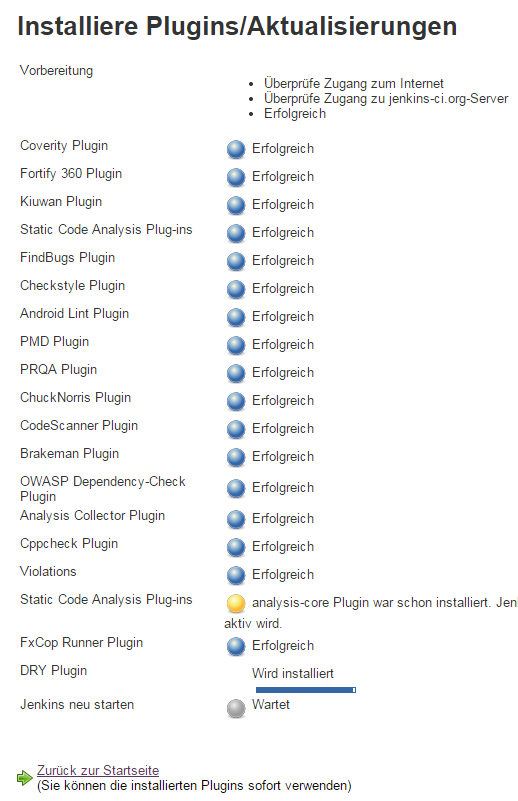
\includegraphics[width=1\linewidth]{img/jenkins-code-analysis-plugins.png}
%	\caption{Just a few used Jenkins plugins for static code analysis}
%	\label{fig:jenkins-plugins}
%\end{figure}


\subsection{Teamcity}
\label{subsec:teamcity}
Like Jenkins, Teamcity is a web application for continuous integration, published by the company Jetbrains\footnote{\href{https://www.jetbrains.com/teamcity/}{https://www.jetbrains.com/teamcity/}}. In contrast to Jenkins, its not open source, but freely available with a limitation of 20 build configurations.
Also it claims to be easier to use and configure than Jenkins.
It provides possibilities to run analysers before or after the build process and to inspect resulting reports.
Furthermore, it works together with static code analysers in the commercial IntelliJ\footnote{\href{https://www.jetbrains.com/idea/}{https://www.jetbrains.com/idea/}} IDE from Jetbrains.



\section{Static code analysis in Code Quality Management}
\label{sec:static_code_analysis_code_quality_management}

Code Quality Management (CQM) is the practice of monitoring and controlling the quality of code with different metrics and activities.
Static code analysis is a method of gaining measurements that can be used for CQM. Therefore, CQM tools can benefit a lot by an integration of static code analysis into a common build system.


Advantages and disadvantages of Code Quality Management systems:
\begin{itemize}
	\item[+] Advanced issue management capabilities
	\item[+] Easy integration of additional analysers
	\item[+] Advanced issue visualization
	\item[-] Unintuitive source code provisioning
	\item[-] Increased management overhead for developer
	\item[-] Training for users necessary 
\end{itemize}

Coverity and Fortify, as cloud services, provide beside commercial, sophisticated static code analysis, advanced issue management features and can be seen already as Code Quality Management tools.
Furthermore, CQM, IDE and CI systems can work together, even though there are not many approaches to accomplish this yet. 
Anyway, it is possible to start the analysis in CQM systems continuously over a configuration in a CI tool.
SonarQube is an example for a typical, external Code Quality Management system to run several analysers with different rules on source code.

\subsection{SonarQube}
\label{subsec:sonarqube}
SonarQube\footnote{\href{http://www.sonarqube.org/}{http://www.sonarqube.org/}} is an open source project, implemented as web application within its own web server, with the aim to monitor, analyse and manage the quality of source code. 
Besides analysis against common coding guidelines, like duplicate code, missing comments and potential bugs, it also checks with an own rule engine (Squid) for several security issues (e.g. from the OWSASP Top 10 list).
Therefore it provides a central place to manage intuitively analysis rules from different analyser extensions.
The main difference to CI tools, is the feature to manage the found issues.
Over plugins it is possible to extend the analysis scope to over 20 programming languages.
Finally it is even possible to start a SonarQube Analysis over Jenkins with the corresponding Jenkins plugin\footnote{\href{http://docs.sonarqube.org/display/SONAR/Configuring+SonarQube+Jenkins+Plugin}{http://docs.sonarqube.org/display/SONAR/Configuring+SonarQube+Jenkins+Plugin}}  or with a plugin in the Eclipse IDE\footnote{\href{http://docs.sonarqube.org/display/SONAR/SonarQube+in+Eclipse}{http://docs.sonarqube.org/display/SONAR/SonarQube+in+Eclipse}}.



\section{Evaluation}
\label{sec:evaluation}
We decided to make a qualitative evaluation, with usability inspection heuristics described in the book Information Visualization by Kerren et al. \cite{InformationVisualizationBook}.
From the work of Hollingsed et al. on 15 years of usability inspection evaluation \cite{15yearsUsabilityEvaluation}, we derived the best method would be a combination of a cognitive walk-through, combined with the usability heuristic evaluation defined by Nielsen \cite{Nielsen:UsabilityInspectionMethods}.
This wide-used, informal, very cost efficient and effective method is proven to find with a appropriate skilled evaluator team 55 - 90\% of all usability problems.


The usability inspection over heuristic evaluation method uses a small group of usability experts, who evaluate a
user interface using a set of guidelines and noting the severity of
each usability problem and where it exists. 
We combine it with a cognitive walk-though, in the way, that three experts go through the tools with a cognitive expected path in context of applying static code analysis with an additional usability guidelines list for every stage.


\subsection{Walk-through stages and evaluation questions}
\label{subsec:walkthrough}

We identified four stages of our walk-through and evaluate several usability guidelines in each stage:

\subsubsection{Prepare analysis}
\label{subsubsec:evaluation_prepare}
\begin{itemize}
	\item \textit{Is the tool easy and intuitive to configure?} \\
	In this question, we appraise how complicated it was, to set the continuous integration environment up and create a test project with our test source.
	
	\item \textit{Is it possible to add external analysers?} \\
	This is a very useful feature, maybe even elementary. Not being able to add external analysers means that only the included analysers can be used.
	
	\item \textit{Is it possible to configure the analysers?} \\
	Configuring static code analysers is mandatory. For example, there is a huge trade of between accuracy and speed. Accurate analysis can result in very high computational costs. Keep in mind that the analysis is supposed to run for each commit. If an analyser run takes hours, this would not be practical anymore.
	
	\item \textit{Is it possible to view the rules?} \\
	This question targets the transparency of the used static analysers. It can be very helpful to be able to view all supported rules if you want, for instance, check if a specific feature is checked or not. Additionally, viewing the rules can help to understand why an issue was reported and how the code can be improved.
	
	\item \textit{Is it possible to choose, add, edit, delete rules?} \\
	This is related to the previous question, but goes a little further. Imaging you got ascertain that at specific flaw is not detected by a static code analyser. In case, the analyser supports the editing of the used rule-set, you can simply add a custom rule or edit an existing one.
	
	Choosing (selecting) only a subset of all existing rules can result in a faster analyser run which can come in very handy if frequent analysis should be performed, e.g. at each commit and thereby multiple times a day.
\end{itemize}


\subsubsection{Run analysis}
\label{subsubsec:evaluation_run}
\begin{itemize}
	\item \textit{Is it easy and intuitive to start the analysis?} \\
	How much effort is required to manually start an analysis? Is this even possible or are only automated analyses supported? Furthermore, starting an analysis can be easy as a click on a website or hard like a manual invocation of a specific command on the source code folder on some server.
	
	\item \textit{Is it possible to following the analysis progress?} \\
	This can be useful if an analysis takes some time and the process cannot be determined in a different way. Also, the analyser output can be helpful for debugging purposes.
\end{itemize}


\subsubsection{Evaluate analysis results}
\label{subsubsec:evaluation_results}
\begin{itemize}
	\item \textit{Is there an issue overview with severity levels?} \\
	An overview over the the amount of issues of different severity classes is the best starting point for bigger projects to investigate the impediments and code problems of the project.
	
	\item \textit{Is it possible to view an issue trend/history?} \\
	Especially for bigger projects it is important for the management to get a visual history about the change of code quality, the risks and amount of security problems in the project, to take mitigation actions, like coding guideline trainings, etc. soon enough, to keep the code secure and robust.	
	
	\item \textit{Is there a mapping from issue to source code position?} \\
	Perhaps one of the most important features of an analyser is the mapping of an issue, to a concrete row and column in the code.
	This helps the developer to find and identify the problem and makes it much easier to resolve the issue.
	
	\item \textit{Is there a description for every issue?} \\
	The description of the issue, optimally with examples, is also very important, if the developer has no awareness of the problem.
	It helps to understand the issue and serves as educational helper, to avoid the same issue in the future.
	
	\item \textit{Is the issue description easy to understand with solution suggestions?} \\
	Corresponding to the question before, a description can also contain possible solutions to the issue, that might be helpful to resolve the problem faster.
	
	\item \textit{Is there a possibility to filter issues? (severity, category, tag, ...)} \\
	For projects with many issues it is important to filter for the most important ones, to speed up code reviews, to find the most common issue categories and to prioritize issues.
\end{itemize}


\subsubsection{Manage analysis results}
\label{subsubsec:evaluation_manage}
\begin{itemize}
	\item \textit{Is it possible to assign issues to developers?} \\
	Analysis results serve as input for code reviews. Such reviews need to get managed and scheduled and therefore an important feature is the possibility to assign issues to developers.
	
	\item \textit{Is is possible to edit issues status? (Resolved, False positive, ...)} \\
	Since many analysers report false positives or duplicate issues, it is important to mark issues as resolved or false positive to prevent code review overheads.
\end{itemize}


\subsection{Eclipse}
\label{subsec:evaluation_eclipse}

Eclipse is an open source and extensible Integrated Development Environment (IDE). It is easy to add plugins which can make development environment more customizable. It does not provide any built-in feature for static code analysis. However, this can be achieved by installing some available plugins. Adding additional plugins to eclipse is sometimes not an easy task. It could take a lot of time for configuring and exploring the third party tools. There are available analysers that provide best effort vulnerabilities detection and code analysis.

Once installation of any analyser is done, than it is easy to run analysis on the code. Analysis process usually runs in background and it cannot be seen. After the process finishes, results can be seen on the console. Reporting capabilities are not much more informative. Only very generic information is available about the defects detected during the analysis process. However, issues' severity levels, their mapping to source code and general description is made available by the tools. There is no possibility to add or change the analysis rules. Furthermore, it is not possible in this environment to modify issues' status, assignment to developer, filtering and viewing issues' histories.
\subsection{Jenkins}
\label{subsec:evaluation_jenkins}

\begin{figure}[t]
	\centering
	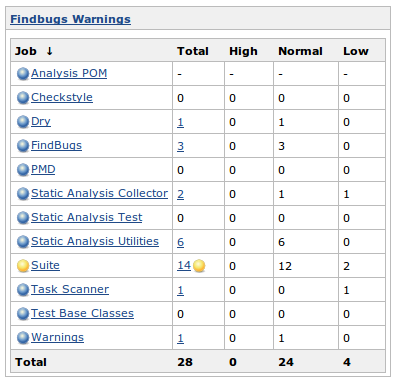
\includegraphics[width=0.45\textwidth]{img/jenkins_dashboard.png}
	\caption{Jenkins Dashboard using the common ``Static Code Analysis Plug-ins'' plugin that combines the results of multiple analysers.}
	\label{fig:jenkins-dashboard}
\end{figure}

Jenkins itself has no static code analysis included but a major feature of Jenkins is its extensibility. Including a code analysis step in a build process is simple as adding a \textit{build step}. The analysers configuration can be passed by command line options or via a configuration file, depending on the used analyser. How well an analyser can be configured or if the rule-set can be modified depends not on Jenkins but only on the analyser. We can, therefore, make no statement about this.

Starting an analysis in Jenkins is easy as pressing the respective button in the web interface. The process can be watched live in a self-reloading page that prints all console output that is made by all build steps. Since static code analysis is just a build step in Jenkins, the output of the analysers is visible there too.

Visualization of analysis results is done by free plugins only. In general, the analyser creates a result file that is written to a specific location. After the build is done, the relevant plugins check the project root for those result files and parse their content. Therefore, the way the results are shown depends largely on the quality of the used plugin. Nevertheless, one common static code analysis plugin exists\footnote{\href{https://wiki.jenkins-ci.org/display/JENKINS/Static+Code+Analysis+Plug-ins}{Jenkins: Static Code Analysis Plug-ins}}, that is able to collect the results of multiple plugins and create a common overview over all results, see figure \ref{fig:jenkins-dashboard}. Again, the quality of this visualizations depends hardly on the quality of the available plugins for a specific analyser. We observed a good support and an ordinary visualization quality but these information is only founded on samples.




\subsection{Teamcity}
\label{subsec:evaluation_teamcity}


The installation of Teamcity, consisting of a web server and a database and was as easy as in Jenkins, but assisted by an installation wizard, hence slightly easier. 
Since it is also a highly customizable CI, it supports every programming language and only the externally used static code analyser are language dependent.


But the extensibility is the biggest difference to Jenkins.
Even popular analyser like FindBugs and PMD are not available as plugins and need to run externally as stand-alone version.
During the build process it is possible to start the external analysers and or import the XML reports of those analysers.
Teamcity as a JetBrains product, has a binding to the popular IntelliJ IDE from JetBrains.
This IDE is out of scope for our work, but contains own static code analysers and the main difference of handling static code analysis in Teamcity to Jenkins, is the fact, that Teamcity rely on the analysis reports produced by IntelliJ. 
For our evaluation we had to install and configure the analysers FindBugs and PMD externally as stand-alone version and import the results during the build process in Teamcity.
Hence, it is not possible to manage rules at a central instance and much effort to install, configure and run different analysers with custom rule-sets.


Since there are no static code analysers integrated in Teamcity, the issue presentation from the XML report is just a non-user-friendly, parsed XML tree of issues with analyser dependent information. In the case of FindBugs and PMD, with a short description and reference to the line of code.
There is no filter, sort or search option for severity levels or categories and also no issue management capabilities.
The only positive aspect of this view, is the issue position link, with an IntelliJ hook, to directly jump to the line of code, where the issue is located in the project, if the IntelliJ plugin is installed.


Compared to Jenkins, Teamcity has a more modern user interface, the build process is easier to configure, but lags on plugins for static code analysis and is coupled to other commercial products like the IntelliJ IDE.


\subsection{SonarQube}
\label{subsec:evaluation_sonarqube}

The last evaluated tool was the CQM system SonarQube.
SonarQube consists out of 3 parts: a webserver, a database to load and store analysis results and the SonarQube Runner, which analyses the code specified in a project property file.
There was no easy installation wizard to install those parts, hence it had a higher installation effort compared to the other evaluated tools.
Especially the task of starting the analysis, was very unintuitive and accompanied by manual creation of a property file in the file system for specifying project and source code parameters.
The starting of the analysis was much easier in the other tools and it would be desired to create the property file and start the analysis within SonarQube.


SonarQube is easy extensible and supports more than 20 programming languages over additional plugins, hence we had no problems to evaluate its code analysis capabilities with our Java test project JEdit.
Beside the build-in analyser, it is possible to add additional analysers like FindBugs and PMD.


The most impressive feature, is the intuitive and central rule management in SonarQube, that allows to configure custom rule sets, so called Quality Profiles, from a pool of rules from different analysers, categories, severity classes and tags.
It provides an easy way to create custom analysis profiles for special purposes, to focus on the most important issues and to increase the performance.
The rules have a clear structure, with description, severity class, category etc. and it is even possible to add additional information or solution suggestions to the rule descriptions.
Unlike the tested CI and IDE tools, SonarQube even comes with security relevant default rules e.g. derived from OWASPTop10 and CWE vulnerabilities, that can easily be combined with rules from external analysers like FindBugs and PMD.


\begin{figure}[t]
	\centering
	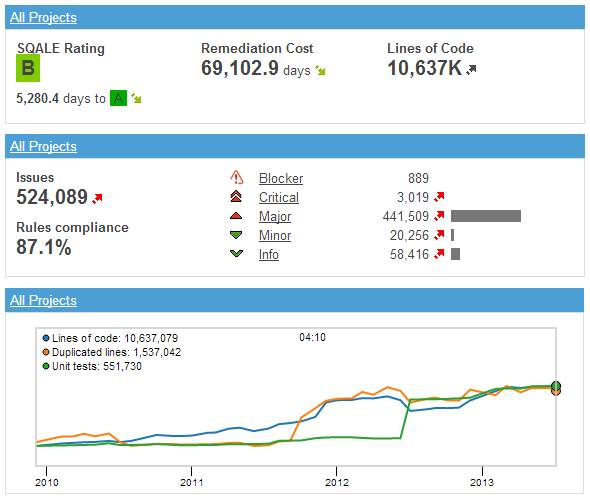
\includegraphics[width=0.45\textwidth]{img/Sonarqube.png}
	\caption{A part of the SonarQube Dashboard that shows the most important measurements and analysis results for all projects}
	\label{fig:sonarqube-dashboard}
\end{figure}


The dashboard of SonarQube as starting point presents an overview for one or all projects with different informative metrics, mostly for code quality, e.g. lines of code and duplicate lines of code, but also gives a rating of the project depending on the found issues and other metrics.
As seen in figure \ref{fig:sonarqube-dashboard}, it shows the number of issues of the different severity levels (Blocker, Critical, Major, Minor, Info), the rule compliance and a trend graph of the project for different metrics.
Additionally a table with the most violated rules and resources can be displayed and the number of issues for different issue states.
One of the main differences of CQM systems to CI systems or IDE's, are the detailed capabilities of managing issues, e.g. assigning issues to developers, assigning issues different states like open, closed, false positive, confirmed, etc. 
In the menu Issues and Issue-Drilldown it is possible to manage the issues, to sort the issue list, search for issues matching to specific rules and get more information to the issue and most important where the issue is located in the code.


The only experienced drawback was in the issue management.
In the Rule-Management one can filter rules by tags and categories (bugs, security bugs), but it is not possible to use those filters in the issue management. 
This leads to a big list of issues where e.g, unused code issues and security issues can't be distinguished anymore.



\subsection{Comparison}
\label{subsec:comparation}

After evaluating all above mentioned tools with different configuration, we have come up with some results which can be seen in figure \ref{fig:comparison_matrix}. While preparing analysis environment; Eclipse allows installation of additional plugins, but does not support the customization of analysers. Teamcity also comes up with same capabilities and restrictions like eclipse. On the other hand, most promising features are addressed by SonarQube, which include from easy installation and configuration to customization of analysers. Moreover, it is easy to run analysis from Eclipse and Jenkins user interfaces, but other tools are not so much user friendly in this regard.

When talk about reporting capabilities, Eclipse provides issues' description, their mapping to source code and severity levels. Jenkins presents results with same characteristics like eclipse but additionally allows issues' history and filtering. Teamcity has the worst demonstration that only includes description of results. While, SonarQube has the best visualization approach. It covers all features of Eclipse and Jenkins as well as it offers suggestions for individual bugs. Last but not the least, SonarQube is the only tool that can give the opportunity to delegate issues and modify their status.

\begin{figure*}[t]
	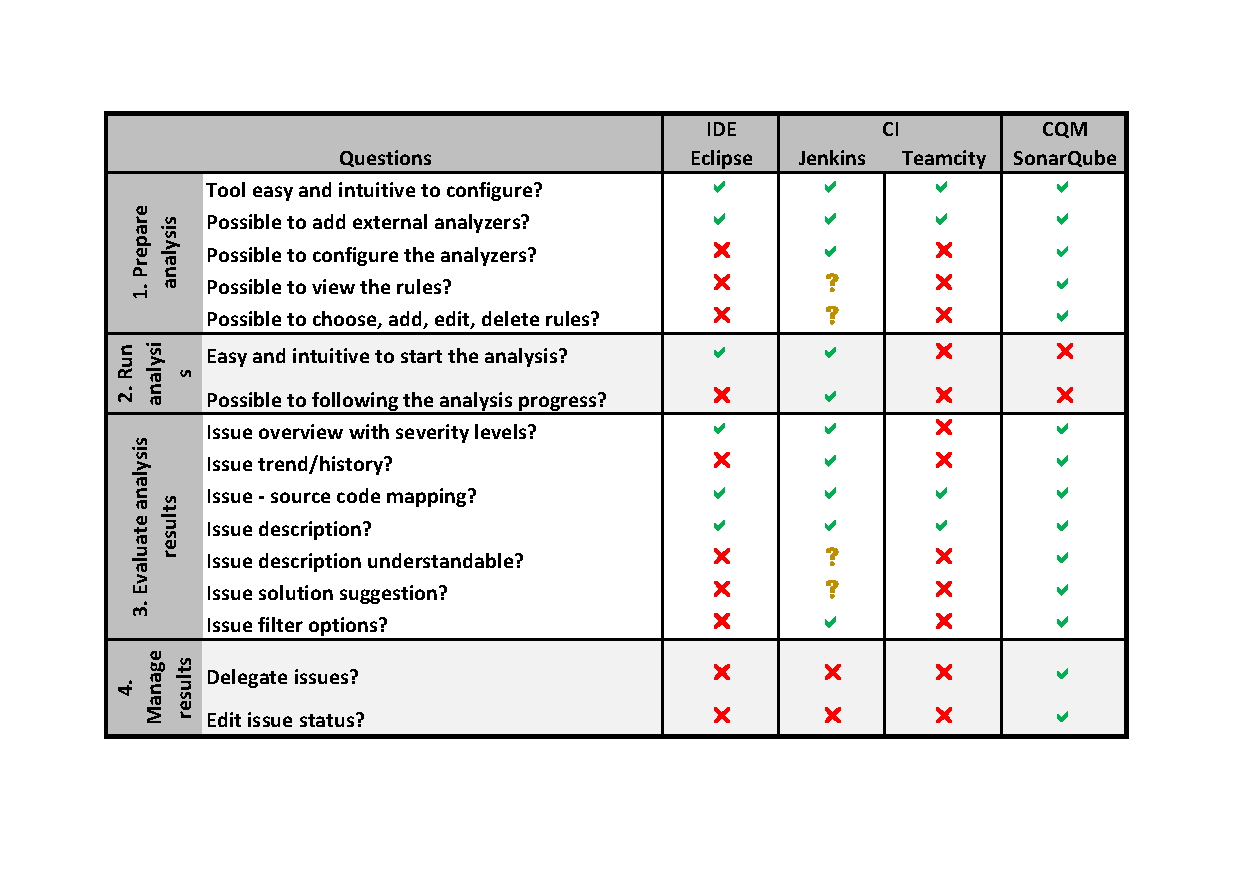
\includegraphics[width=\textwidth]{img/comparation}
	\caption{Comparison Matrix.}
	\label{fig:comparison_matrix}
\end{figure*}

\section{Conclusion}
\label{sec:conclusion}
	%\item Conclusion about how input validation is done in frameworks, what can be better ...
Its really not that easy to find the right static code analyser for your project with a specific programming language. There are lot of open source tools, but very old and just supported by Jenkins over hacks. static code analysers need to be customized to find special problems (like Java Vulnerabilities). Is it better to integrate static analysis in Jenkins or in IDE or in Code Quality Management tools? Is reporting in Jenkins usable? No...just in combination with Code Quality Management tools like SonarQube, Coverity, ... and the analysis in those tools can be triggered in CI tools, but it is much effort to configure.
Future work: Using many tools is basically a good idea, because more tools find potentially more vulnerabilities. A future approach would be to implement a tool that can filter all the generated reports. Thereby duplicate vulnerabilities findings can be merged and false positives can be reduced.


\bibliographystyle{IEEEtran}
% argument is your BibTeX string definitions and bibliography database(s)
\bibliography{references}

\end{document}


